\documentclass[a4paper]{article}

\usepackage[spanish]{babel}
\usepackage[utf8]{inputenc}
\usepackage{amsmath}
\usepackage{graphicx}
\usepackage{hyperref}
\usepackage[colorinlistoftodos]{todonotes}

\title{Inteligencia Artificial potencia la Exploración en Marte}

\author{Anthony Bladimir Vélez Villavicencio}

\date{\today}

\begin{document}
\maketitle

\begin{abstract}
Desde tiempos antiguos, el ser humano ha sentido una profunda curiosidad por conocer más sobre el planeta en el que vivimos, así como sobre la posición que ocupamos en el sistema solar. Impulsados por esa curiosidad, descubrimos que la Tierra no es el único planeta en nuestro sistema, sino que hay otros similares, algunos más cercanos y otros más distantes. Esto genera preguntas como: ¿podría existir vida en esos planetas? ¿Estarán habitados por seres similares a los humanos? Estas interrogantes han motivado los viajes espaciales, comenzando con la misión a la Luna, el cuerpo celeste más cercano a la Tierra, donde el hombre logró pisar su superficie con el apoyo de la tecnología desarrollada. Las imágenes obtenidas del planeta Marte muestran que es similar a la Tierra y que podría haber albergado vida. La ciencia ha sido fundamental en la búsqueda de señales de vida, pero para avanzar es imprescindible el apoyo de la Robótica y la Inteligencia Artificial. Los robots, a diferencia de los humanos, no necesitan comer, beber o dormir, lo que permite que las misiones espaciales sean más eficientes en la recolección de información. Un ejemplo de ello es "Mars Express", la sonda espacial robótica de la Agencia Espacial Europea que realiza labores de exploración en Marte.
\end{abstract}

\section{Introducción}


Desde que se tomó la primera fotografía detallada de Marte en 1965, las misiones de sondas espaciales al planeta rojo han revelado un mundo que, aunque nos resulta extrañamente familiar, presenta diferencias suficientes para desafiar nuestras ideas sobre el funcionamiento de los planetas. Cada nuevo descubrimiento sobre Marte nos obliga a replantear nuestras teorías previas. A primera vista, Marte parece ser más comprensible: al igual que la Tierra, posee casquetes polares, nubes en su atmósfera, patrones estacionales, volcanes, cañones y otros rasgos geológicos reconocibles. Sin embargo, las condiciones en Marte difieren drásticamente de las que conocemos en nuestro propio planeta.

En las últimas tres décadas, las sondas espaciales han mostrado que Marte es un desierto frío, rocoso y estéril bajo un cielo rosado brumoso. Sin embargo, el paisaje marciano actual sugiere un pasado violento, con volcanes en erupción, cráteres creados por meteoritos y torrentes de agua que inundaron su superficie. Cada aterrizaje o maniobra orbital de las sondas nos sigue despertando la curiosidad. Una de las preguntas clave en la exploración de Marte es: ¿existe vida en Marte? Entre los descubrimientos más destacados está la posible presencia de agua líquida, ya sea en su pasado remoto o preservada en el subsuelo. La presencia de agua es crucial, ya que, en la Tierra, donde hay agua, hay vida. Si Marte alguna vez tuvo agua líquida o aún la conserva, surge inevitablemente la duda de si pudo haber desarrollado vida microscópica. ¿Existen pruebas de vida pasada en Marte? De ser así, ¿podrían algunas de esas diminutas formas de vida existir todavía hoy? ¡Imaginen lo emocionante que sería confirmar un "sí"!

Aun si no hay evidencia de vida en Marte, sigue habiendo motivos para emocionarse. Los seres humanos podríamos llegar a ser esa "vida en Marte" si algún día decidimos viajar allí. Mientras tanto, aún queda mucho por aprender sobre este intrigante planeta y sus extremos ambientes. Para desentrañar las posibilidades de vida en Marte, pasada, presente o futura, la estrategia del programa de Marte se ha enfocado en "Seguir el agua". Esto requiere comprender el entorno actual de Marte y examinar características como los lechos de ríos secos, el hielo en los polos y tipos de rocas que se forman solo en presencia de agua. Debemos investigar posibles fuentes de aguas termales, fumarolas hidrotermales o reservas de agua subterránea. También buscamos averiguar si Marte alguna vez tuvo un gran océano en su hemisferio norte, como sugieren algunos científicos, y cómo pudo haber cambiado de un ambiente acuoso a la árida desolación que vemos hoy.

Para responder a estas preguntas, es esencial adentrarnos en la historia geológica y climática del planeta, descubriendo cómo y por qué Marte sufrió cambios tan drásticos. Cada misión futura deberá seguir principios científicos rigurosos que evolucionarán conforme sigamos haciendo nuevos descubrimientos.








\begin{figure}
\centering
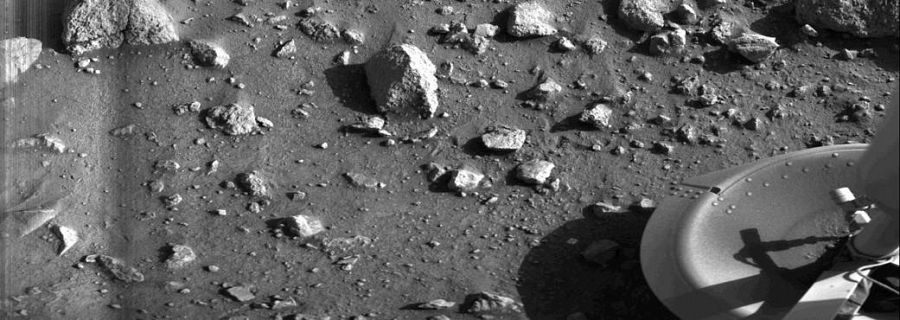
\includegraphics[width=0.7\textwidth]{fotoMarte.jpeg}
\caption{\label{fig:frog} Primera fotografia de Marte}
\end{figure}


\section{DESARROLLO DE LA INVESTIGACION }

El Centro Europeo de Operaciones Espaciales (ESOC) ha implementado la Inteligencia Artificial (IA) para apoyar a la sonda Mars Express de la ESA en su misión de buscar indicios de vida en Marte, ya sea presente o pasada. Desde 2004, la sonda ha utilizado avanzados instrumentos para estudiar la atmósfera, superficie y subsuelo marciano, confirmando la existencia de agua y buscando señales de vida. Debido a que la sonda genera una gran cantidad de datos científicos, estos deben ser transmitidos a la Tierra de manera precisa para evitar su pérdida, ya que la memoria a bordo es limitada y se sobrescribe constantemente. Anteriormente, este proceso era gestionado por software que requería la supervisión humana para programar la transmisión de datos y eliminar aquellos que podrían perderse, lo que era un proceso lento y con riesgo de pérdida de información valiosa.

Desde 2005, investigadores del Instituto Italiano para la Ciencia y la Tecnología Cognitiva (ISTC-CNR) y el equipo de ESOC han estado desarrollando MEXAR2, una herramienta de IA que optimiza la gestión de datos, planificando inteligentemente qué información podría descartarse y generando los comandos necesarios para su transmisión. Esta solución ha logrado reducir prácticamente a cero la pérdida de datos y ha disminuido en un 50% la carga de trabajo del equipo de planificación, permitiendo optimizar el uso del ancho de banda y liberar tiempo para otras misiones.

El éxito de MEXAR2 ha motivado a los científicos de ESOC e ISTC-CNR a explorar nuevas aplicaciones de IA, como el proyecto "RAXEM", que optimiza el envío de comandos a la sonda. Estas tecnologías también se aplicarán a futuras misiones, como ExoMars, la primera misión europea en enviar un vehículo robótico a Marte. Según Donati, estos avances abren la puerta a un mayor nivel de autonomía en futuras misiones de la ESA.


\begin{figure}[h!]
    \centering
    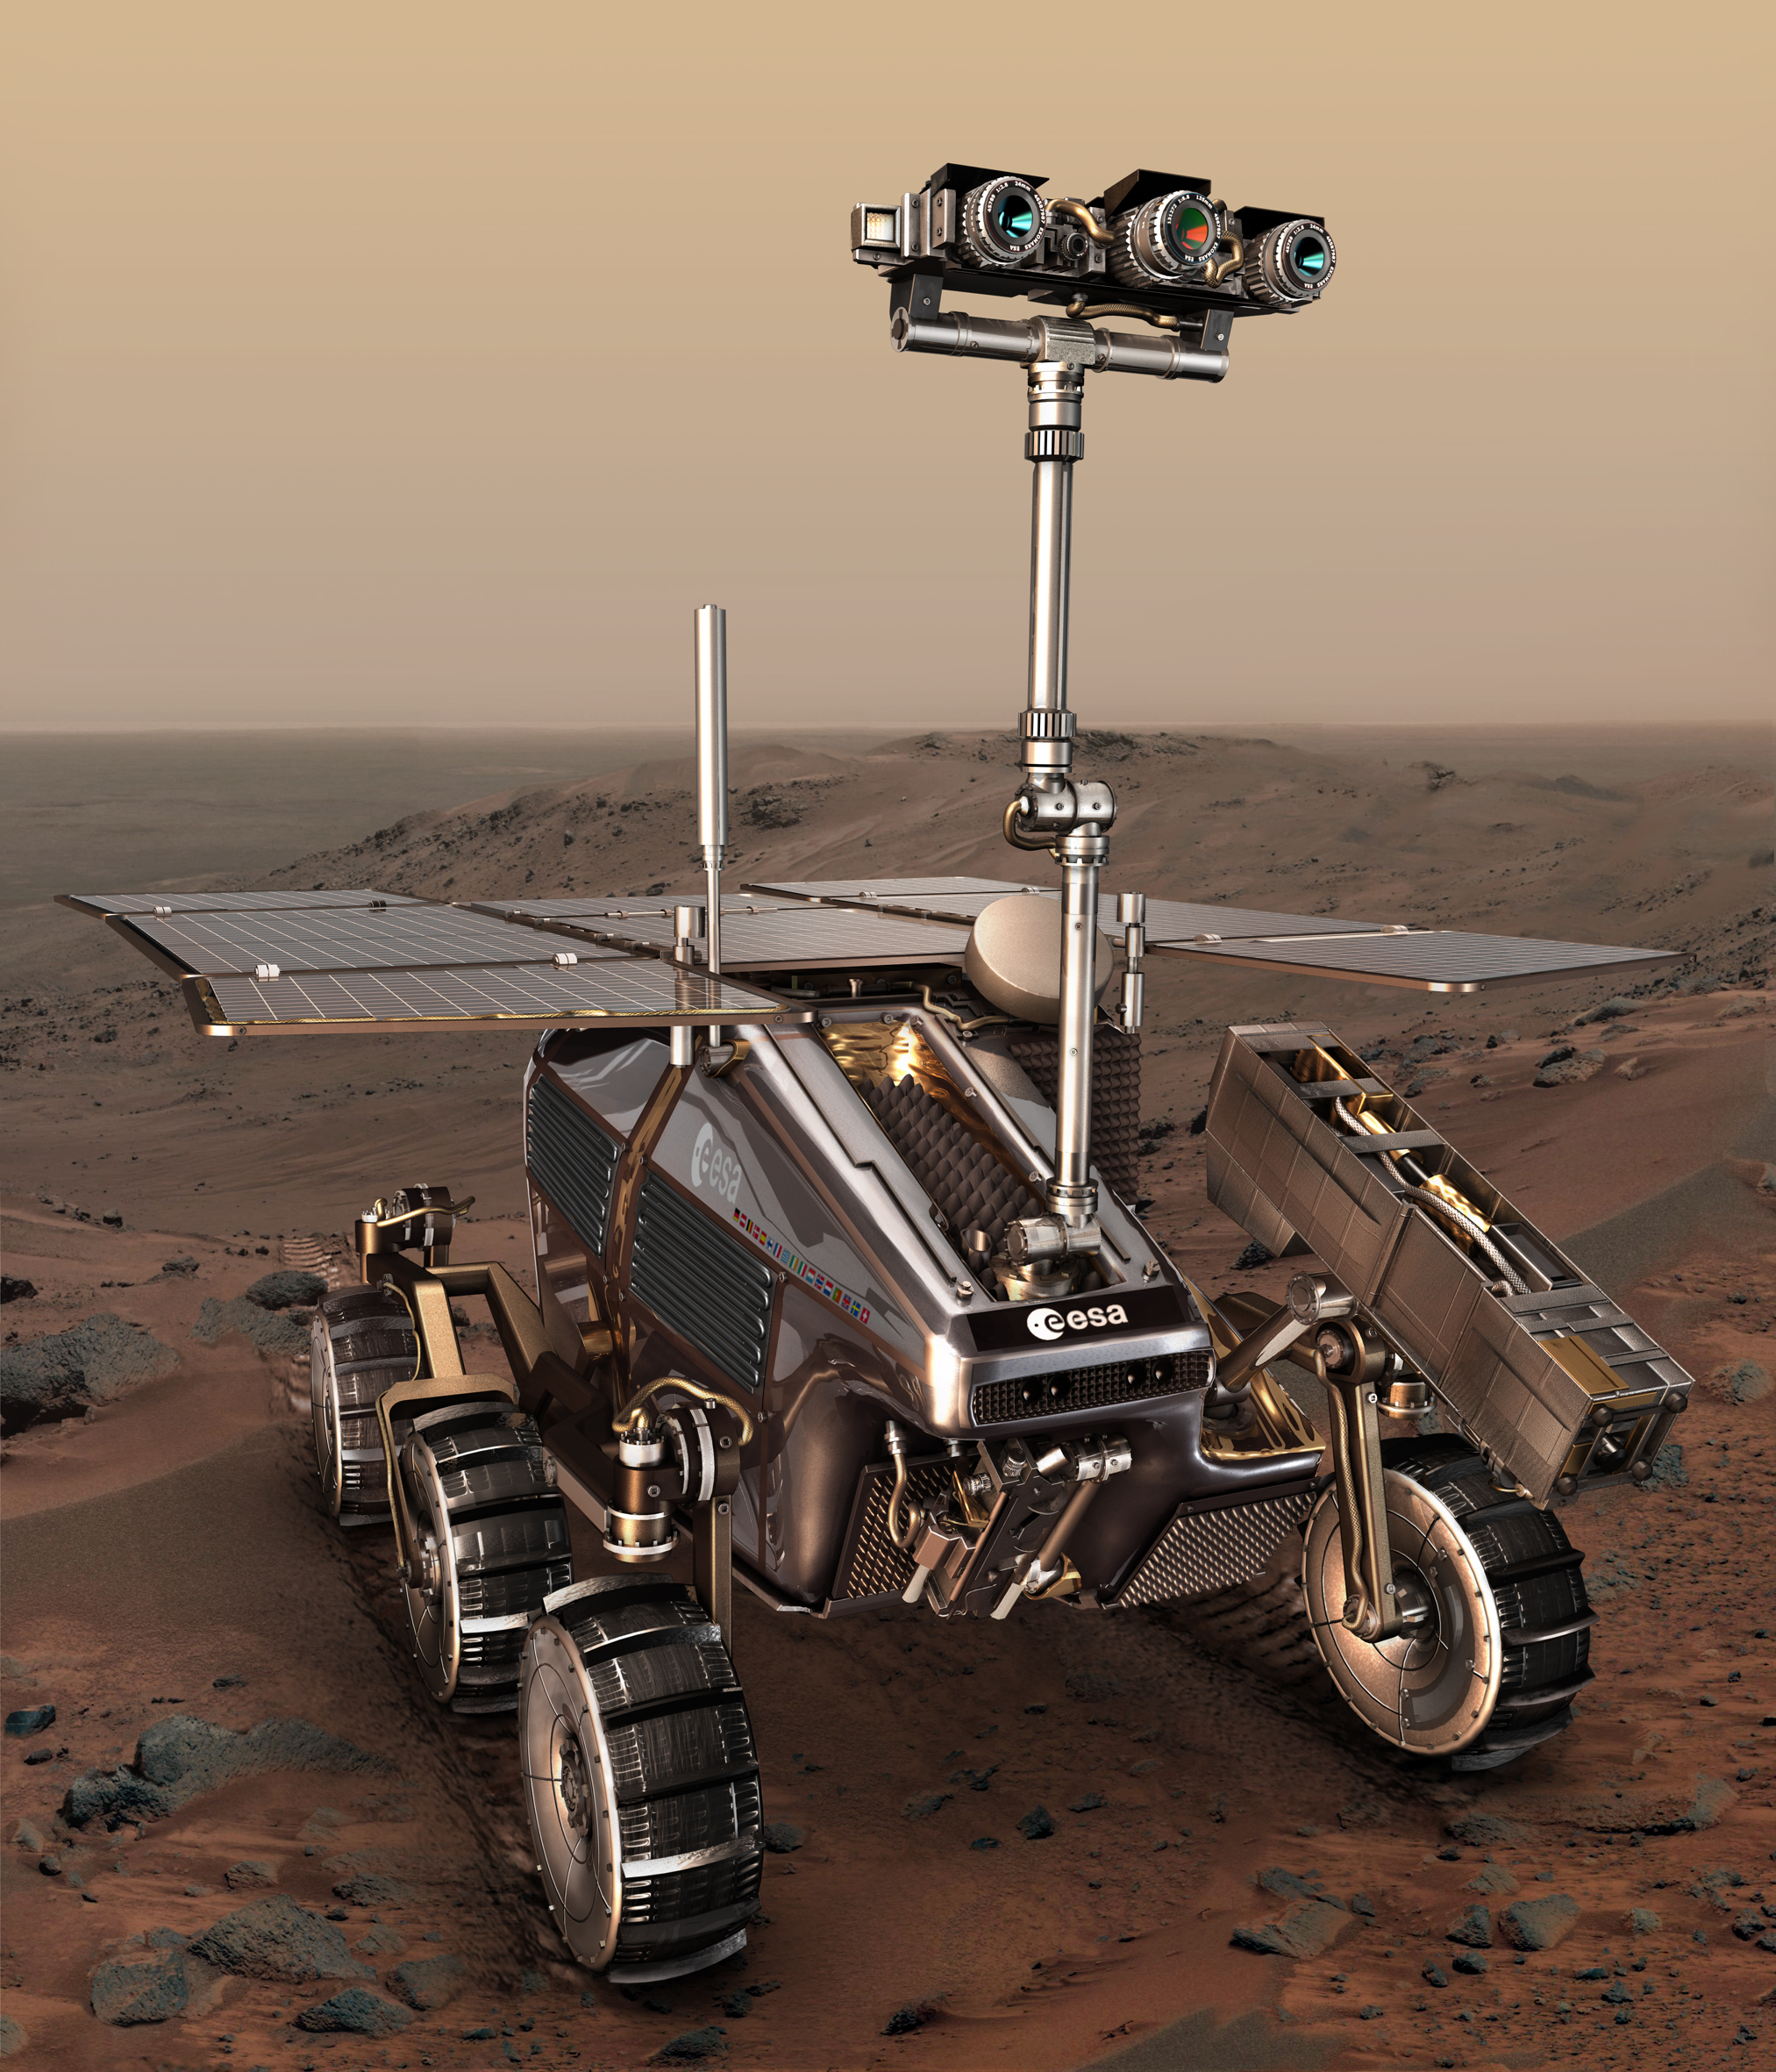
\includegraphics[width=0.5\textwidth]{Exomarsrover_high.jpg}  % Especifica la ruta de tu imagen
    \caption{Robert}  % Texto opcional debajo de la imagen
\end{figure}

% Texto con enlace al video
\begin{center}
    Robert: \href{https://www.youtube.com/watch?v=k0rbV8mAiCY&ab_channel=MarteEspa%C3%B1ol}{Haz clic aquí para ver el video}
\end{center}

\section{APLICACIONES }
\textbf{Mars Express estudia los depósitos más misteriosos de Marte}

El radar de la sonda Mars Express de la ESA ha revelado nuevos detalles sobre la formación Medusae Fossae, uno de los depósitos más enigmáticos de Marte. Se han obtenido por primera vez mediciones directas sobre la profundidad y las propiedades eléctricas de estos materiales, aportando nuevas pistas sobre su origen. Estos depósitos, ubicados cerca del ecuador marciano, podrían ser relativamente jóvenes debido a la escasez de cráteres en la zona, lo que contrasta con áreas más antiguas. Entre 2006 y 2007, Mars Express utilizó su radar MARSIS para estudiar la región, revelando la profundidad de las capas al medir el tiempo que tardaban las señales de radar en atravesarlas y rebotar en la roca subyacente.

Thomas Watters, del National Air and Space Museum, señala que antes de estos estudios se desconocía el verdadero grosor de los depósitos de Medusae Fossae. Los datos de MARSIS también mostraron que estos depósitos tienen propiedades eléctricas que sugieren que podrían estar compuestos por material suelto y polvoriento, aunque resulta difícil explicar cómo un material tan poroso podría tener varios kilómetros de espesor sin compactarse bajo el peso de las capas superiores. Aunque las propiedades eléctricas son similares a las del hielo, no hay evidencias claras de la presencia de hielo en las regiones ecuatoriales de Marte. Jeffrey Plaut, del Jet Propulsion Laboratory, explica que si hubiera hielo, debería estar enterrado a varios metros de profundidad, ya que las bajas presiones en Marte provocarían su rápida evaporación si estuviera cerca de la superficie. Por lo tanto, el origen de la formación Medusae Fossae sigue siendo un misterio.

Los estudios con MARSIS también han revelado detalles del subsuelo marciano, mostrando antiguos cráteres de impacto ocultos bajo las llanuras del hemisferio norte, lo que sugiere que, aunque la superficie es joven y lisa, la corteza subyacente es muy antigua. Estos hallazgos proporcionan nuevos indicios sobre la historia geológica de Marte, destacando las diferencias entre sus hemisferios norte y sur.


\begin{figure}
\centering
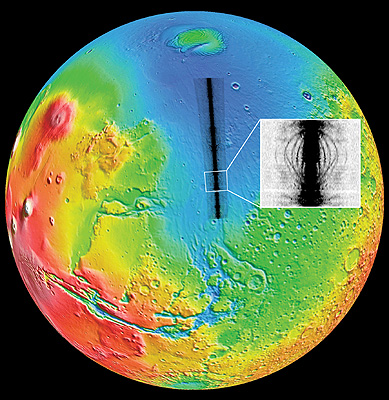
\includegraphics[width=0.5\textwidth]{marte-express.jpg}
\caption{\label{fig:frog}  Marte bajo la superficie.}
\end{figure}

\section{Conclusiones}
Desde que se tiene conocimiento de Marte en nuestro sistema solar, la posibilidad de vida en el planeta rojo ha generado incertidumbre, debido a su semejanza con la Tierra. La exploración de Marte ha sido constante en busca de indicios de vida, dado que se cree que podría haber agua, lo cual incrementa la probabilidad de que exista vida. No obstante, todo el conocimiento actual no habría sido posible sin las herramientas y tecnologías modernas, donde la Inteligencia Artificial y la Robótica juegan un papel crucial. Estos avances tecnológicos han sido fundamentales para llegar al punto en el que estamos hoy. A medida que la tecnología continúa evolucionando, es probable que se obtenga más conocimiento sobre otros planetas y el origen del universo, e incluso se logre determinar si existe alguna forma de vida en otros lugares del cosmos.

\section{Bibliografía }



\begin{itemize}
\item Rojas Castillo Franz, Inteligencia Artificial potencia la Exploración en Marte, 2008.\end{itemize}





 



\end{document}